\chapter{Semantic Connections Theory}
\label{SemanticConnectionsTheory}

\begin{flushright}{\slshape    
Essentially, all models are wrong, but some are useful.} \\ \medskip
    --- George Box \cite{Box1987}, statistician
\end{flushright}



%begin TiiS

Extracting from the lessons learned during the three design iterations, a theory was developed for interacting with a system of devices in a ubiquitous computing environment. This chapter introduces a theory of semantic connections, in which the connections and associations between devices play a central role. Semantic connections focus on the semantics---or meaning---of the connections between entities in a smart environment. 

The theory may be used to analyse (i.e. understand, explain and predict) what happens with interaction events and other interaction data when devices are interconnected and form an ecology of smart objects. As an introduction to the Semantic Connections theory, we first focus on the Semantic Connections user interaction model.

\section{User interaction model}
\label{InteractionModel}

A user interaction model for semantic connections is shown in Figure \ref{model}. It describes the various concepts that are involved in the interaction in a smart environment and shows how these concepts work together. The interaction model was inspired by the \ac{MCRpd} by Ullmer and Ishii \cite{Ullmer2000} which in turn was based on the \ac{MVC} model, both of which are described in Section \ref{mcrpd}. 

\begin{figure}
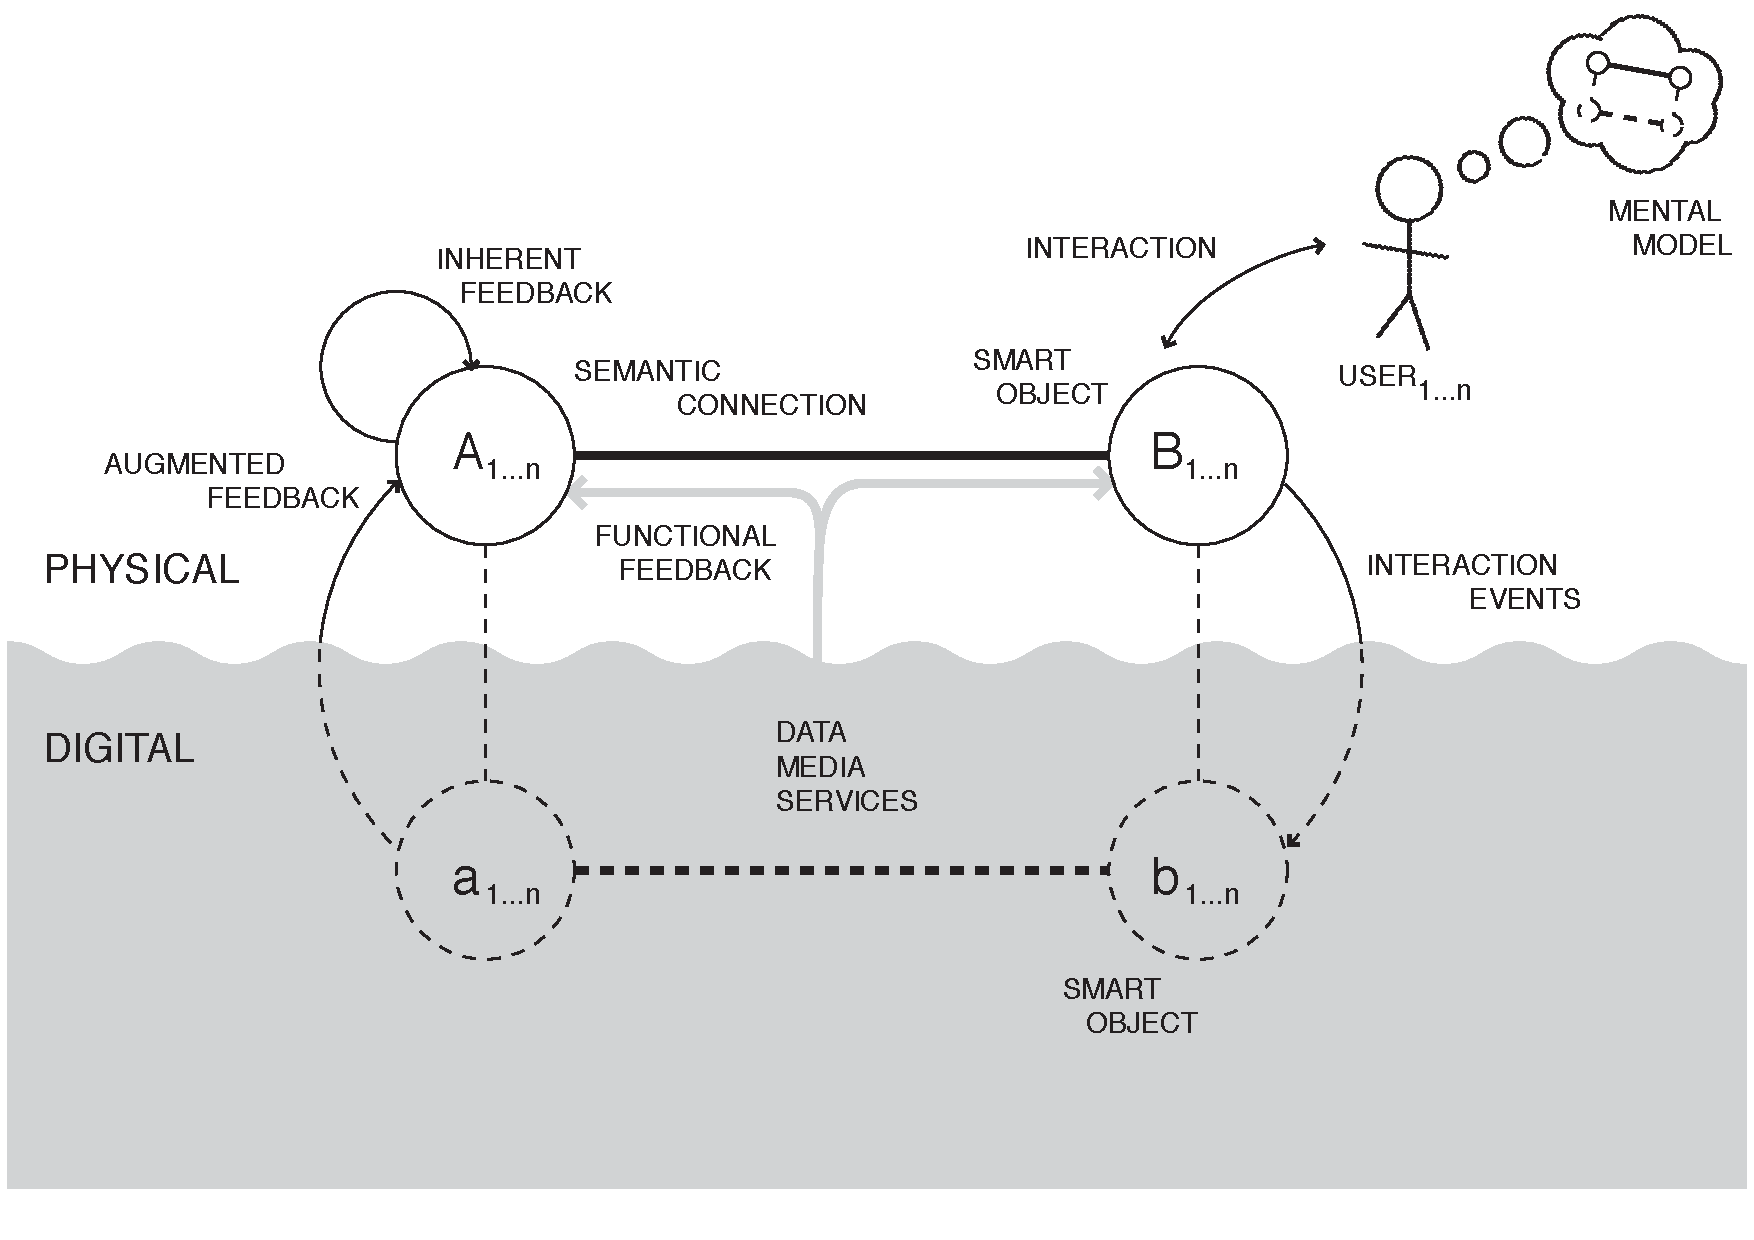
\includegraphics[width=\columnwidth]{InteractionModel}
\caption{Semantic connections user interaction model}
\label{model}
\end{figure}

\marginpar{The terminology of inherent, augmented and functional feedforward and feedback is adopted from \cite{Wensveen2004} and was previously introduced in Section \ref{interactionFrogger}.} 
We first distinguish between the physical and digital domains of the user interaction. A user does not observe directly what is happening in the digital domain, but experiences the effect it has in the physical world by interacting with various smart objects. Semantic connections exist between these objects. By interacting with the objects, users create a mental model of the system that they are interacting with, which only partly includes the digital domain. The digital part manifests itself in the physical world as data, media and services. 


When a user interacts with a smart object, he/she senses feedback and feedforward, directly from and inherent to the controls of the device (inherent feedback), digital information augmented onto the physical world (augmented feedback) and perceives the functional effect of the interactions (functional feedback).\marginpar{Note that in Figure \ref{model} the arrow on the left shows the feedback (or output) of the smart object, and on the right it shows the input (the interaction event). This to avoid repetition, as they may and in most cases will, occur on both sides.} The user actions in the physical world are transformed into interaction events and device state changes. This interaction data in terms of user intentions is stored in the smart space. The notion of a smart space means that data are stored either by an information broker or the smart objects themselves, and can be accessed by the other smart objects in the smart space. We use the term smart environment as a broader term to refer to both the digital and physical spaces, which include both the smart space and the smart objects.

% possibly together with user preferences, defaults and context information.






% In figure (TODO fig vertical view) we describe how user actions with smart objects on the physical lever are translated into interaction events in the digital domain. As user actions are transformed into events, we use the (Nielsen's model) to describe the level along the continuum. 
% 
% To enable user interaction in smart spaces on the level that was sketched in the introduction, the developer community needs to agree on a way of describing the various elements involved in the interactions. These interaction elements or controls are physical by nature (i.e. they are material parts or at least directly perceivable in the physical world), which means that their physical meaning and some of physical properties need to be preserved while describing them. In the sections that follow sections we propose the concepts of interaction primitives (Section \ref{InteractionPrimitives}) and interaction events (Section \ref{InteractionEvents}) as ways to describe these elements and their interactions.
% 
% \begin{figure*}[hbt]
% \centering
% 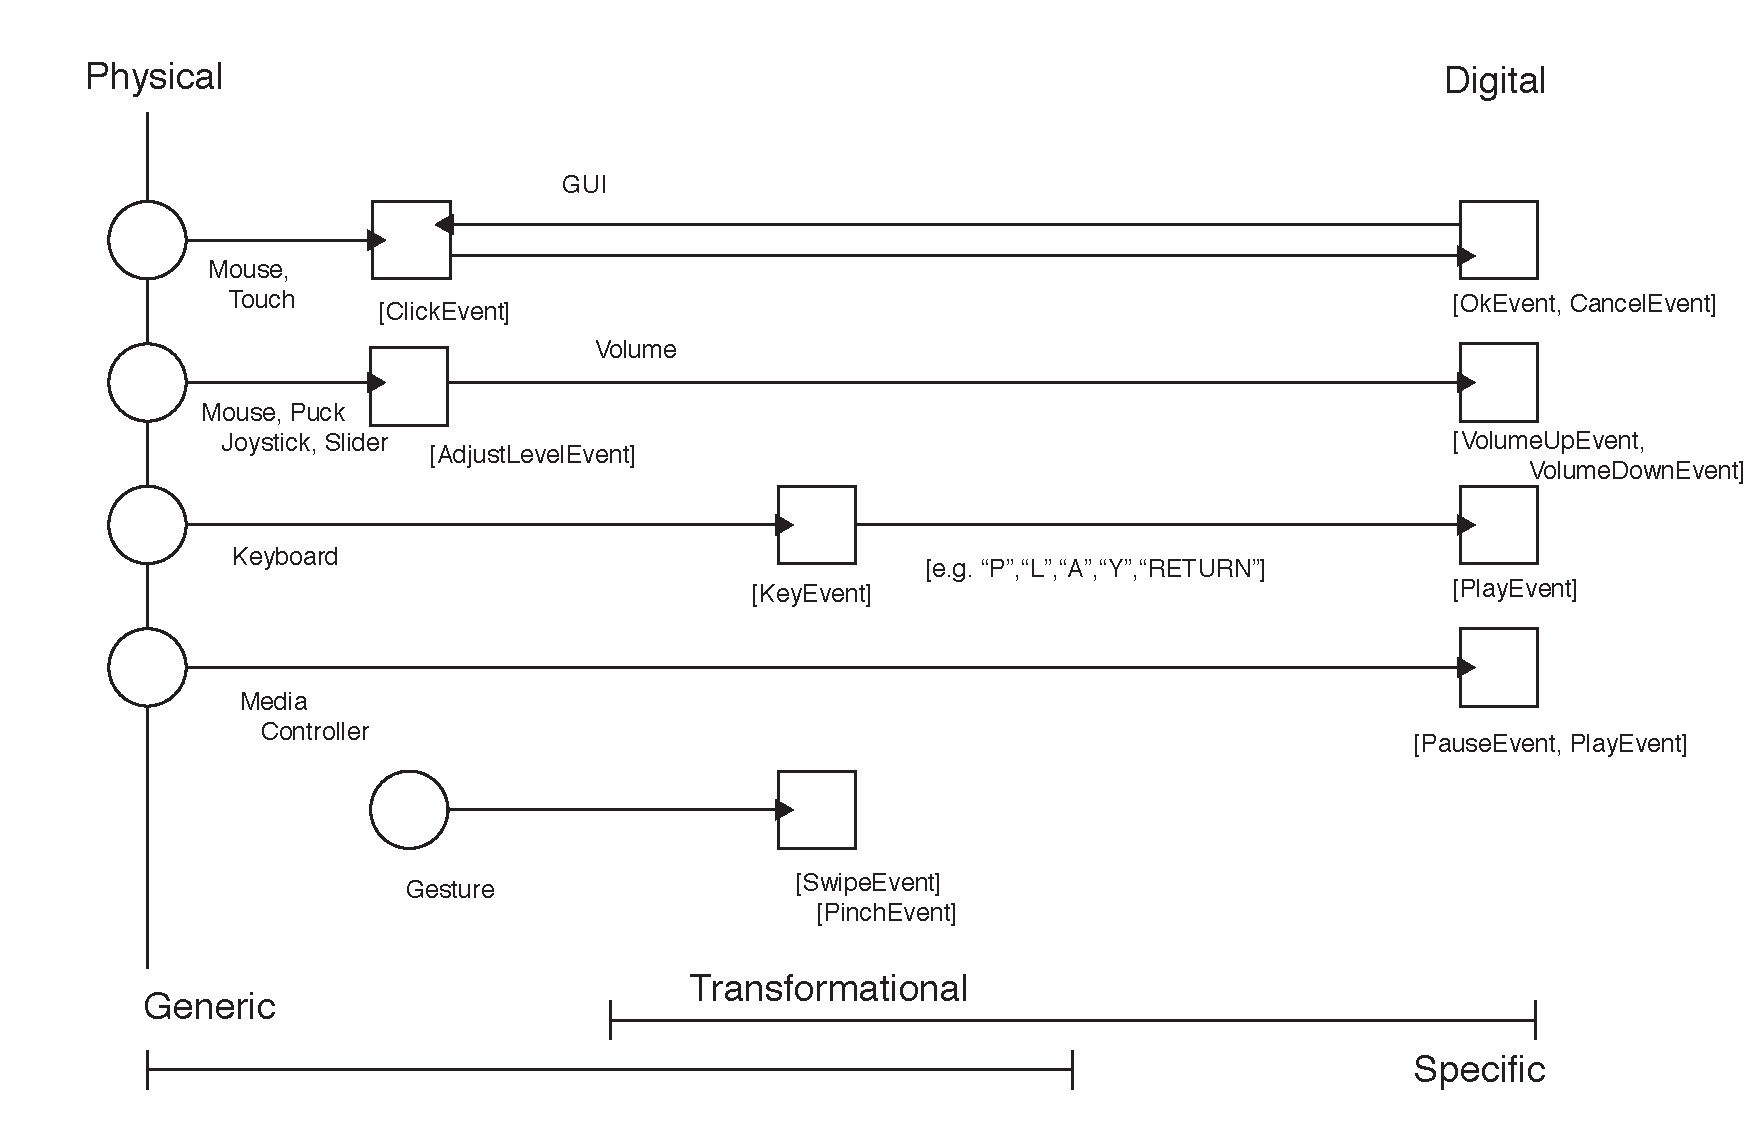
\includegraphics[width=400px]{UserInterfaceModel}
% \caption{User Interface Model}
% \label{interfaceModel}
% \end{figure*} 
% 
% Figure \ref{interfaceModel} shows our proposal to model user interfaces in terms of their physical, real-world interaction properties (like position, movement, rotation, force and torque) and their transformation towards the consequences they have in the digital domain (e.g. triggering interaction events, changing states). The entities represented in the model as circles are what we call \emph{interaction primitives}, the smallest addressable interaction element that has a meaningful relation to the interaction itself. 
%
%On the left-hand side of the figure we plot entities that sense \emph{physical} properties like position, movement or pressure. We consider these properties to be very \emph{generic}, as they do not report a user's intention directly. The inputs first need to be transformed into an intentional event (events that express user intention). This can happen directly, for example pressing a play button, which is transformed into an \texttt{PlayEvent}. It can also follow a series of intermediate transformational steps, where a sequence of interaction events (possibly happening on different devices) may be used to capture the user's intent. This sequence of events is then transformed into a single intentional event.
%
%On the right-hand side of the figure we have the \emph{digital} entities that represent the intentional events. We consider these entities to be very \emph{specific}, as they communicate the (assumed) intention of the user's actions directly.
%
%Entities and their relationships in an interaction together form an \emph{interaction path}. The interaction exchange or action between elements in the path is conducted via one or more \emph{interaction channels} along which information or action is communicated \cite{dubois_2008}. As an example, a typical interaction path in Figure \ref{interfaceModel} would be: 
%
%\begin{quote}\noindent 
%\texttt{Keyboard}  $\rightarrow$ \texttt{KeyEvent} $\rightarrow$ \texttt{PlayEvent} 
%\end{quote}
%
%while an interaction channel exists between \texttt{Keyboard}  and \texttt{KeyEvent}. 
%
%During the transformation from physical to digital, the interaction devices (or their interaction primitives) also move from generic to more specific, where generic user interfaces start off very generic and stay generic or transformational (meaning they have been transformed but still need further transformation). This means that such interaction devices or interaction primitives can still be transformed into many different events or states. When an interaction primitive travels from generic to specific with a single transformation (like the media controller buttons) it means that that these interaction primitives are very specific UI elements (i.e. have one single function). An example of such an interaction primitive would be a hardware button with a specific label that is only used for one function. As another example, consider a gesture; i.e., a (less) generic interaction primitive that transforms from a physical movement that is sensed in a certain way, to the digital representation of that gesture, being a ``pinch'', ``swipe'' etc. The pinch and swipe are still considered transformational because they still need to be transformed further to result in a certain interaction event. However, in the initial transformation, some meaning is preserved (i.e. the physical characteristics of the gesture). These characteristics limit the number of actual events the gesture can still be transformed into, e.g. a ``swipe right'' gesture should not be transformed into a ``navigate forward'' action, as this is the way we usually navigate backwards. Table \ref{transformationTable} shows some of the possible transformational events we consider to be applicable to smart home environments in which multimedia and lighting devices are connected for certain applications.
%
%\begin{table}
%\centering
%\begin{tabular}{|l|l|}
%\hline
%Event & Entity this event can be performed on\\
%\hline
%AdjustLevel & Volume, Lighting \\
%switchOnOff & Lighting, any SmartObject \\
%Navigate & Playlist, Menu, SequentialData \\
%Undo/Redo & Any interaction event \\
%Stop/Start & Application, Media \\
%DragAndDrop & Media \\
%Query & Media, other events \\
%\hline
%\end{tabular}
%\caption{Examples of transformational events in a smart environment}
%\label{transformationTable}
%\end{table} 
%
%Although describing user interaction capabilities of devices according to the user interface model is valid for user interaction in general, it is specifically relevant when we consider the notion of a smart space through which this interaction data can be exchanged. To achieve this, all events that need to be shared must be modelled in a mutually understandable way. A good way of modelling them would be an ontology, as is shown in section \ref{semanticInteraction}. 
%




\section{Smart Objects}

\marginpar{Note that our definition does not define where the \ac{KP} is situated. For simple smart objects, such as a smart light bulb, the actual \ac{KP} that is communicating to the information broker may be a virtual entity running on any device in the network.}Smart objects are the devices that are connected to the smart space, enabling them to share information with one another. We now define a smart object as follows:

\begin{description}
	\item[Smart Object]A smart object is a device with both computational and network communication capabilities that can be uniquely identified in both physical and digital space.
\end{description}

According to our definition, an \ac{NFC} enabled smart phone is a smart object. A WiFi-connected lamp is also a smart object, given that it can be physically identified, for example by proximity based on signal strength or \ac{RFID}. 

 In terms of our definition, a light switch with an \ac{RFID} tag is not a smart object. A software agent running on a \ac{GUI} (e.g. Microsoft Office's Clippy\footnote{http://en.wikipedia.org/wiki/Office\_Assistant}), is not considered a smart object, even though it is visually perceivable. Despite its apparent physical existence, i.e. physically and digitally identifiable, it is mediated by a computer. In such cases the computer is considered the smart object and not the agent running on it, as the agent is not primarily a physical entity. In the following subsections we describe the concepts specific to the smart objects themselves.

\subsection{Identification}
\label{Identification}
For semantic connections to work in the way they are envisioned in this thesis, a smart object needs to be uniquely identifiable in both the physical and the digital domain. In the physical space it needs to be both user-identifiable and machine-identifiable. A device that is tagged with an \ac{RFID} tag is machine-identifiable in the physical space, and the unique identifier read from this tag is also linked to the digital representation of the smart object. \ac{NFC}---using a near field channel like \ac{RFID} or infrared communication---is an interesting case, because it allows for direct manipulation of wireless network connections by means of proximal interactions \cite{Rekimoto2003}.

Of course, there are many ways in which a smart object may be identified. An IP address makes a device easily identifiable in the digital space, but it is difficult to create a physical representation of this identity. Consider the case where IP addresses are printed on stickers and stuck on computers to make them easier identifiable to IT service personnel. One solution to making these stickers machine-identifiable again is to use \ac{QR} codes, two-dimensional barcodes which can be identified by mobile phone cameras.

\subsection{Interaction primitives}
\label{InteractionPrimitives}

We defined interaction primitives as a way to describe the user interaction capabilities of smart objects in ubiquitous computing environments. \marginpar{Interaction primitives were introduced in Section \ref{sectionSemanticInteractionOntology}.} These interaction primitives are based on the work of Foley, Card and others introduced in Section \ref{interactionTasks}.

The key on a keyboard labelled ``A'' is an interaction primitive, as pressing it not just changes the key's \texttt{Up} state into a \texttt{Down} state, but carries the meaning to \emph{produce} a character ``A''. A gesture \texttt{SwipeLeft} on a touchpad is also an interaction primitive, as this is the smallest addressable element to still have meaning. Describing the input on a lower level would cause it to lose its meaningful relation to the interaction. A touchpad itself is not an interaction primitive but rather an input device. An interaction with the touchpad, annotated with its meaning, can be an interaction primitive. A \ac{GUI} is not an interaction primitive, but a \ac{GUI} element can be.

Interaction primitives are described in terms of their physical properties that are meaningful to a user. For example, an unlabelled button should not only be represented in terms of its \texttt{On} and \texttt{Off} states, but also whether it is in a \texttt{Up} or \texttt{Down} state. This enables the mapping of physical, generic interaction primitives like a rocker switch to specific high-level events like \texttt{VolumeUpEvent}.

An interaction primitive also has a range measure that describes the range of possible values that it can take on. This makes it easier to determine if and how they can be mapped to specific interaction events.

Interaction primitives and interaction events together form an \emph{interaction path} \cite{Dubois2008}. As an example, a typical interaction path would be:
\label{interactionPath}

\begin{quote}\noindent
\texttt{VolumeSliderLeft} $\rightarrow$ \texttt{SlideLeftEvent} $\rightarrow$ \texttt{VolumeDownEvent}
\end{quote}

where the \texttt{VolumeSliderLeft} is an interaction primitive map\-ped to the \texttt{SlideLeftEvent} interaction event. Based on the available context information, this can in turn be mapped to a more specific \texttt{Volume\-Down\-Event}.


% --- The following could be included for more information on interaction primitives (but remember, TODO parts of this chapter africon)

% \begin{figure*}[hbt]
% \centering
% 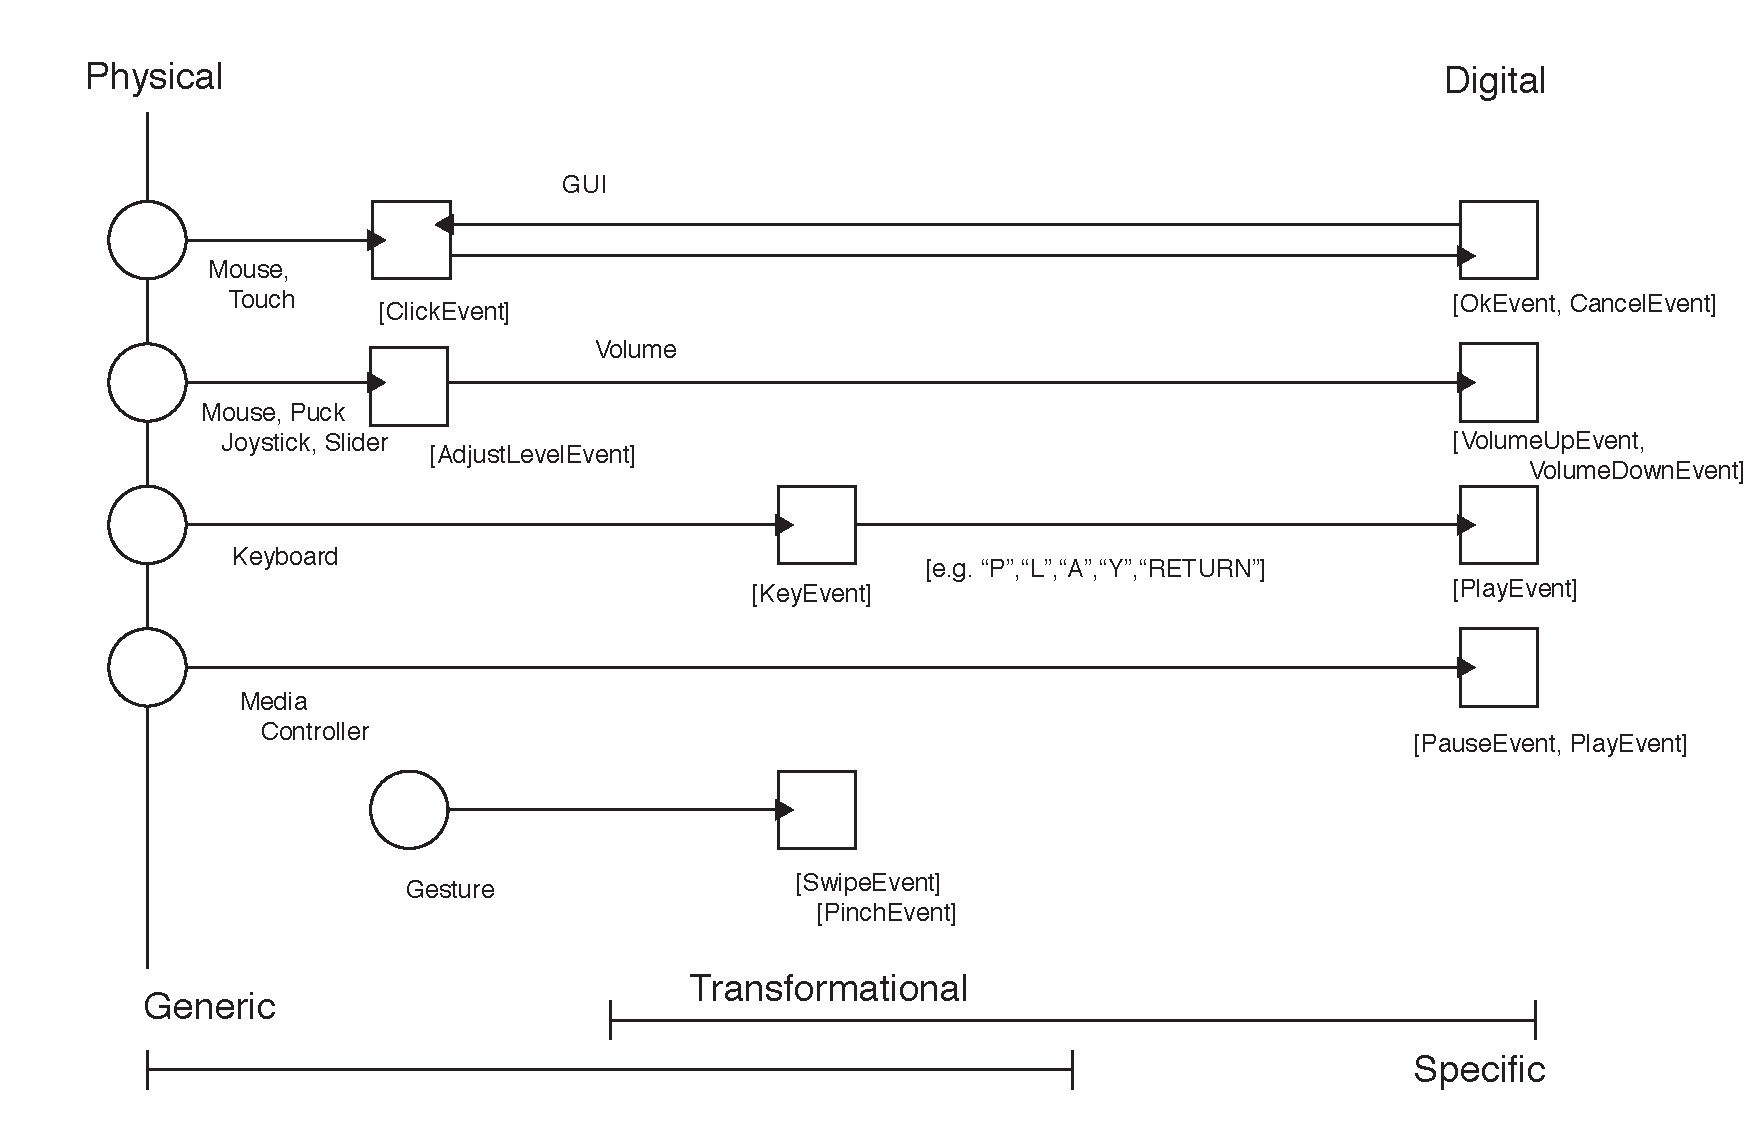
\includegraphics[width=400px]{UserInterfaceModel}
% \caption{User Interface Model}
% \label{interfaceModel}
% \end{figure*} 
% 
% Figure \ref{interfaceModel} shows our proposal to model user interfaces in terms of their physical, real-world interaction properties (like position, movement, rotation, force and torque) and their transformation towards the consequences they have in the digital domain (e.g. triggering interaction events, changing states). Interaction primitives are modelled as circles in this diagram.
% 
% On the left-hand side of the figure we plot entities that sense \emph{physical} properties like position, movement or pressure. We consider these properties to be very \emph{generic}, as they do not report a user's intention directly. The inputs first need to be transformed into an intentional event (events that express user intention). This can happen directly, for example pressing a play button, which is transformed into an \texttt{PlayEvent}. It can also follow a series of intermediate transformational steps, where a sequence of interaction events (possibly happening on different devices) may be used to capture the user's intent. This sequence of events is then transformed into a single intentional event.
% 
% On the right-hand side of the figure we have the \emph{digital} entities that represent the intentional events. We consider these entities to be very \emph{specific}, as they communicate the assumed intention of the user's actions directly.
% 
% Entities and their relationships in an interaction together form an \emph{interaction path}. The interaction exchange or action between elements in the path is conducted via one or more \emph{interaction channels} along which information or action is communicated \cite{Dubois2008}. As an example, a typical interaction path in Figure \ref{interfaceModel} would be:\\
% 
% \noindent 
% \texttt{Keyboard}  $\rightarrow$ \texttt{KeyEvent} $\rightarrow$ \texttt{PlayEvent}\\ 
% 
% 
% while an interaction channel exists between \texttt{Keyboard}  and \texttt{KeyEvent}. 
% 
% During the transformation from physical to digital, the interaction devices (or their interaction primitives) also move from generic to more specific, where generic user interfaces start off very generic and stay generic or transformational (meaning they have been transformed but still need further transformation). This means that such interaction devices or interaction primitives can still be transformed into many different events or states. When an interaction primitive travels from generic to specific with a single transformation (like the media controller buttons) it means that that these interaction primitives are very specific UI elements (i.e. have one single function). An example of such an interaction primitive would be a hardware button with a specific label that is only used for one function. As another example, consider a gesture; i.e., a (less) generic interaction primitive that transforms from a physical movement that is sensed in a certain way, to the digital representation of that gesture, being a ``pinch'', ``swipe'' etc. The pinch and swipe are still considered transformational because they still need to be transformed further to result in a certain interaction event. However, in the initial transformation, some meaning is preserved (i.e. the physical characteristics of the gesture). These characteristics limit the number of actual events the gesture can still be transformed into, e.g. a ``swipe right'' gesture should not be transformed into a ``navigate forward'' action, as this is the way we usually navigate backwards. 

% ---- end


%Table \ref{transformationTable} shows some of the possible transformations we consider to be applicable to smart home environments in which multimedia and lighting devices are connected for certain applications.

% \begin{table}
% \centering
% \begin{tabular}{|l|l|}
% \hline
% Event & Entity this event can be performed on\\
% \hline
% AdjustLevel & Volume, Lighting \\
% switchOnOff & Lighting, any SmartObject \\
% Navigate & Playlist, Menu, SequentialData \\
% Undo/Redo & Any interaction event \\
% Stop/Start & Application, Media \\
% DragAndDrop & Media \\
% Query & Media, other events \\
% \hline
% \end{tabular}
% \caption{Examples of transformational events in a smart environment}
% \label{transformationTable}
% \end{table} 

%Although describing user interaction capabilities of devices according to the user interface model is valid in general, it is specifically relevant when we consider the notion of a smart space through which this interaction data can be exchanged. To achieve this, all events that need to be shared must be modelled in a mutually understandable way. 

%When modelling, only that which is meaningful to be shared with other devices is considered. It is not necessary to describe interactions that are internal to the device and that are not shared.. An accelerometer for example may be modelled as a separate device, sharing the raw accelerometer data to be used by other devices. However, when integrated into smart phones, the accelerometer's data can often be abstracted as part of an interaction path, e.g. to only share the orientation of the device or specific gestures measured with the accelerometer. The raw values may, in this case, need only to be available to the device to be used by the developers of other applications.





% \label{paths}
% \emph{Media paths} connect devices based on their media capabilities, allowing content to be streamed from one device to another. A semantic reasoner is used to perform media type matching, e.g. to determine that a mobile phone, capable of transmitting audio content, can be connected to a speaker system in the room, as it is capable of accepting audio content.
% 
% If two devices share no common media capabilities, it is possible to use a \emph{semantic transformer} to convert the content from one media type to another. An example of a media path is:  
% 
% \begin{quote}\noindent
% \texttt{MediaPlayer} $\rightarrow$ \texttt{SoundToLight\_SemanticTransformer} $\rightarrow$ \texttt{AmbientLighting}
% \end{quote}
% 
% which connects a media player to the ambient lighting in the room via a semantic transformer, converting an audio stream into lighting information (intensity/colour/frequency). This allows the ambient lighting to render the mood of the music played on the media player.

When modelling interaction primitives, only that which is meaningful to be shared with other devices is considered. It is not necessary to describe interactions that are internal to the device and that are not shared. An accelerometer, for example, may be modelled as a separate device, sharing the raw accelerometer data to be used by other devices. However, when integrated into a smart phone, the accelerometer's data can often be abstracted as part of an interaction path, e.g. to only share the orientation of the device, or specific gestures measured with the accelerometer. In this case, the raw values may only need to be available locally on the device, to be used by the developers of other device-specific applications. 


%begin Some Reasoning Required
%From the high-level action that is required, e.g. ControlVolumeUp, first determine which interaction primitives are required by mapping to basic functionality (for example requires a GenericBoundedSlider or GenericBoundedKnob with range 0-100), then determine the required mapping function (e.g. mapping TODO get correct mapping function, where v is the sensed value with some constant C), and  then look at what devices in the area can provide this control, show possibilities, then allow for creating a connection between the device/control and the user action.
 
%Possible things that need to be inferred:
% What can be inferred based on these descriptions of interaction primitives?  We could, for example, infer input devices types based on their properties:
% 
% \begin{itemize}
% 	\item If an interaction primitive measures position in one dimension, we can infer that it is a type of \texttt{Slider}.
% 	\item If a phone has a \texttt{Slider} and a speaker has \texttt{Volume} functionality we can infer that these devices can be connected, where the one device is used to control the volume of the other device.
% 	\item By describing a computer mouse in terms of its manipulation operators and possible states (measuring movement on x,y-axis and states {Up,Down}), we can infer it to be a \texttt{Slider}, \texttt{2DTablet} or a \texttt{Button}.
% \end{itemize}

%end Some Reasoning Required

One of our academic partners in the \ac{SOFIA} project, the University of Bologna, created an independent implementation of our interaction primitives \cite{Bartolini2011}. % , which was published in the Springer Journal of Personal and Ubiquitous Computing



\section{Semantic Connections}

%TODO Semantic connections as an interaction metaphor to handle data flow

%begin TiiS

\emph{Semantic connections} is a term we introduced \cite{VanderVlist2010,VanderVlist2010a} to describe meaningful connections and relationships between entities in an ecosystem of interconnected and interoperating smart objects. 

% (see design iteration 1)


% The digital counterparts of semantic connections are modeled in an ontology. There may be very direct mappings, e.g. a connection between two real-world entities may be modelled by a \texttt{connectedTo} relationship in the ontology. Semantic connections can exist between the following entities: artifacts, smart objects, sensors, UI elements, places, (smart) spaces and persons. Semantic connections have properties like directionality, symmetry, transitivity, reflexiveness and modality.

%Crucial to our approach is to make the gap between user goal and action smaller. If we consider streaming music from one device to another, ``streaming'' now consists of multiple actions that do not necessarily make sense to a user, but are necessary from a technological perspective. In our view, this single high-level goal should have one single high-level action, or at least as few actions as possible. The actual configuration of the devices, i.e., matching device capabilities, transforming content or information to the format that is accepted by the receiving device and negotiating passwords and permissions should happen automatically, based on the user's goals and the constraints of the environment. Our earlier work on mapping the user needs to the actual configurations of the devices uses an heuristic approach at mostly syntactic level \cite{Feijs2004,Hu2006}. In this work this is improved by the semantic transformers. In the following two sections we describe how to model device capabilities and relate them to user actions through the use of semantic transformers.

%\begin{definition}
%A semantic connection is a relationship between two entities in a smart environment that can be physically perceived and has meaning to its users. The semantic connections stands for a functionality emerging from the connection in the physical world, which is technically achieved by connectivity technologies and protocols at the lower level, in the digital domain
%\end{definition}

%not sure about this yet

\marginpar{Semantic connections were introduced in Chapter \ref{DesignIteration1}.}
The connection between a remote control and a wirelessly controllable (on/of or dimmable) light bulb is a semantic connection. The connection exists between two smart objects that can be physically identified and connected through physical proximity. The connection's communication technology is unknown to its user and the remote control and light are conceptually linked by users, based on the perceived behaviour. 



\begin{figure}
\begin{center}
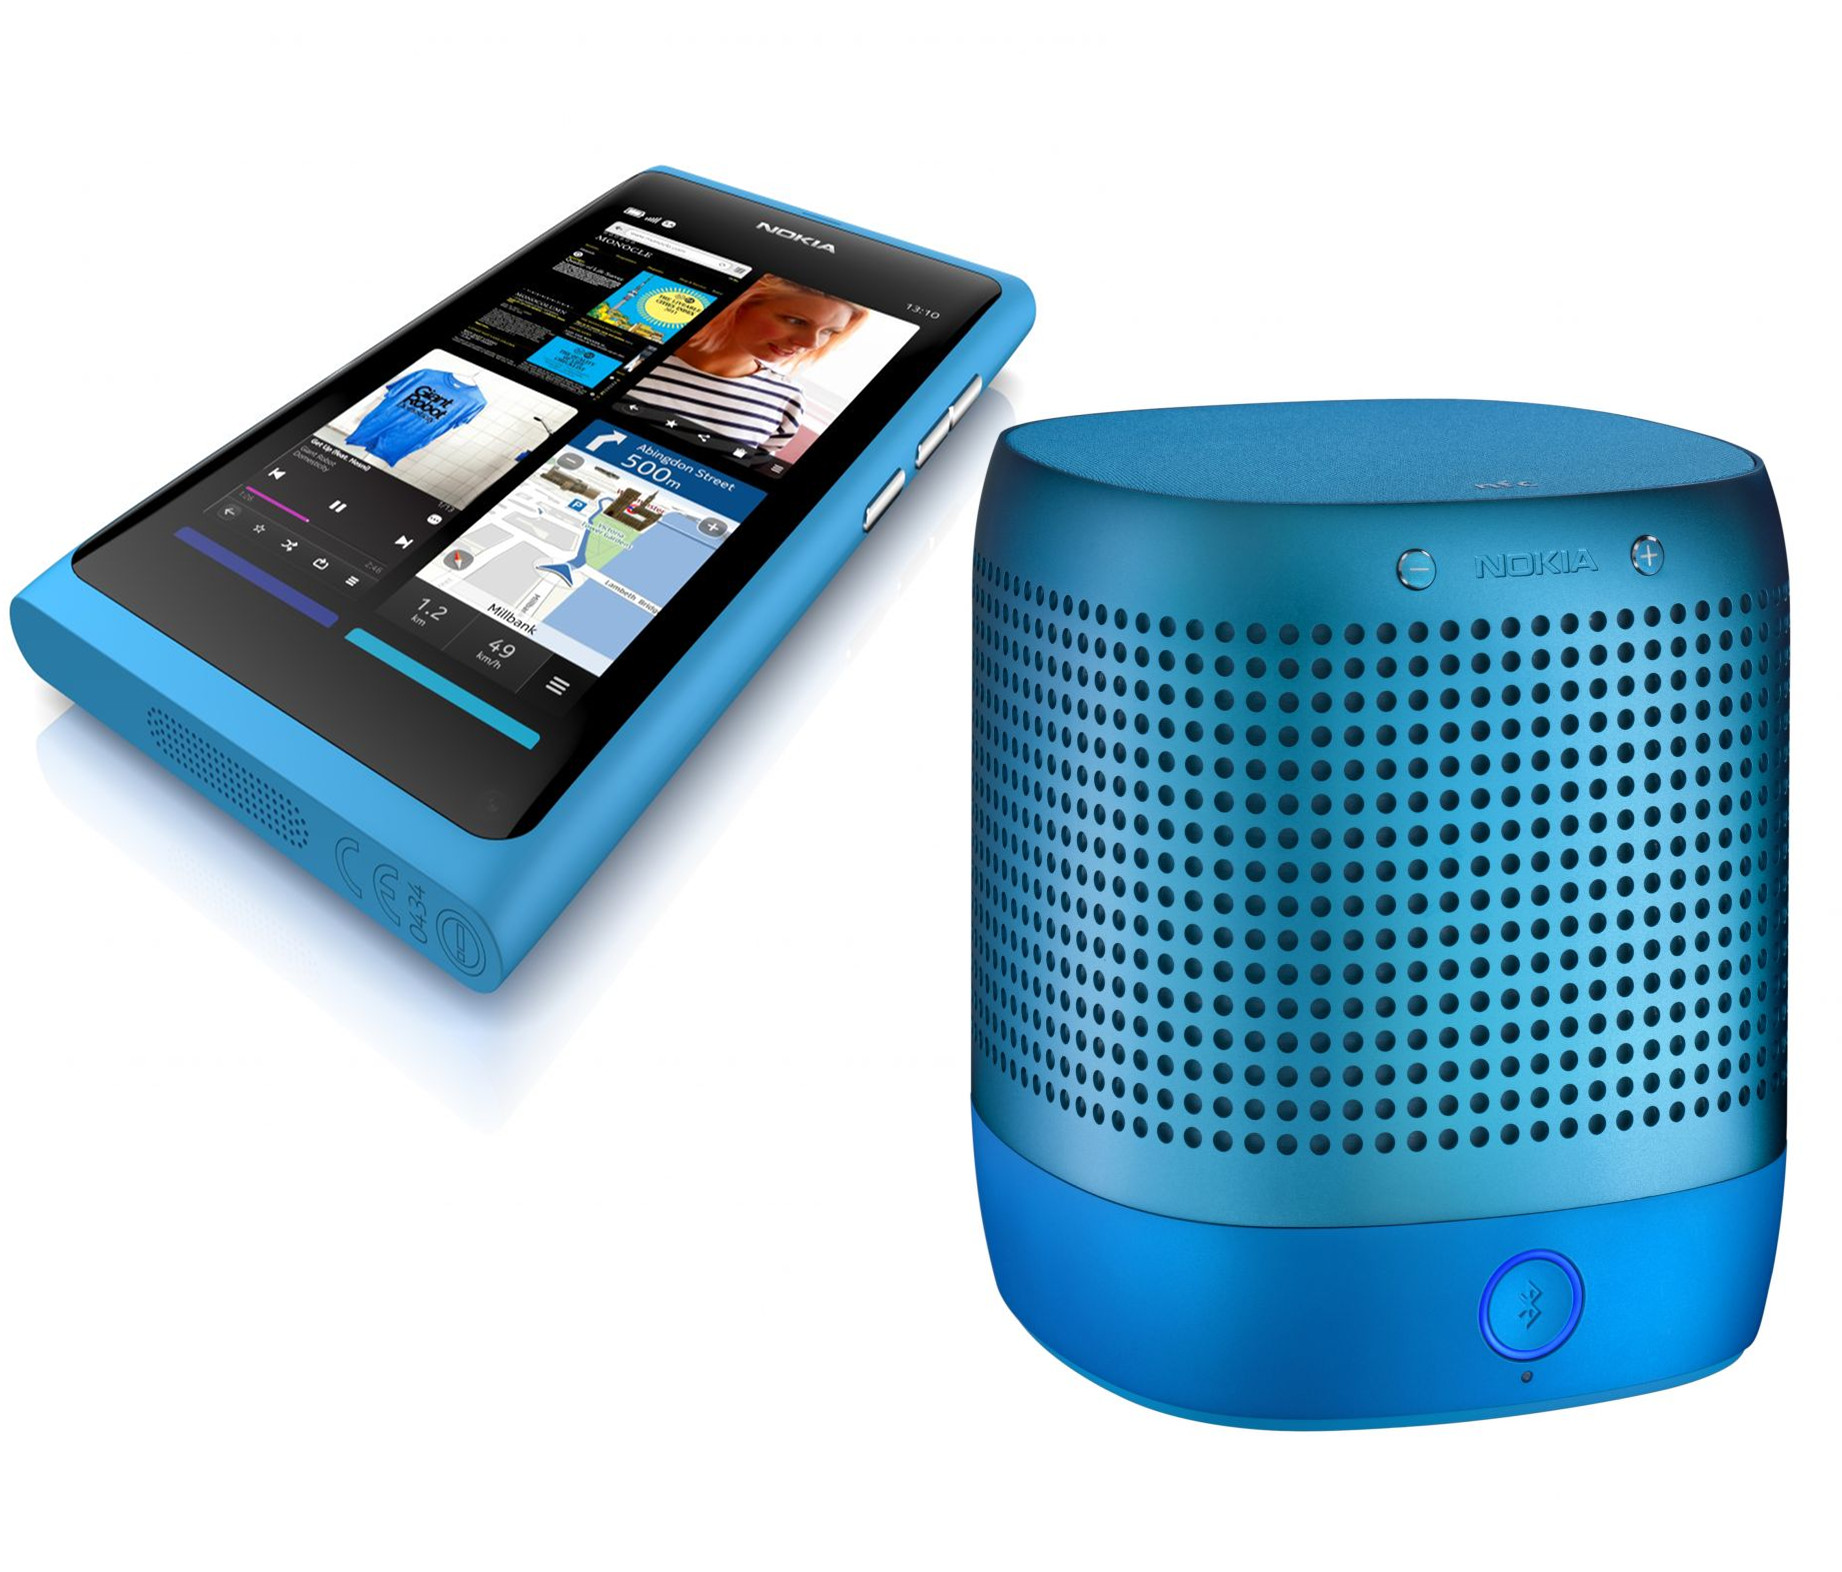
\includegraphics[width=\textwidth]{nokiaplayn9}
\end{center}
\caption{Nokia Play 360$^{\circ}$ speaker system and N9 mobile phone}
\label{nokiaplay}
\end{figure}


Another example of a meaningful connection is the Nokia Play 360$^{\circ}$ speaker system, shown in Figure \ref{nokiaplay}, where music can be streamed wirelessly to the speaker using an \ac{NFC}-enabled smart phone. By touching the phone to the top of the speaker, a connection is created that conceptually ``carries'' the music from the phone to the speaker.

The WiFi connection between a smart phone and a WiFi router is not a semantic connection, as the connection in itself has no clear meaning. A USB cable by itself is also not considered a semantic connection.

Semantic connections make up a structural layer of inter-entity relationships on top of the network architecture. These connections can be the real, physical connections (e.g. wired or wireless connections that exist between devices), or conceptual connections that seem to be there from a user's perspective. 
%The term ``semantic'' refers to the meaningfulness of the connections. We consider the type of connection, which currently often has the emphasis when interconnecting devices (e.g. WiFi, Bluetooth, USB) not to be the most relevant, but what the connection can do for someone---its functionality (e.g. stream music, share files)---even more.
Semantic connections exist in both the physical world and the digital domain. They have informative properties which are perceivable in the physical world. However, some of these physical qualities might be hidden by default, and only become visible on demand by means of a mediating interaction device. The digital parts of semantic connections are modelled in an ontology. There may be very direct mappings, e.g. a connection between two real-world entities may be modelled by a \texttt{connectedTo} relationship between the representations of these entities in an ontology. Sometimes the mapping is not so direct, for example where a semantic transformer is used. Semantic connections have several properties, which are explained in the following subsections. 

%The rationale behind Semantic Connections is to rely on:
%\begin{itemize}
%\item the meaning of existing objects to provide meaning for the relationships between the objects and the resulting meaning of the networked objects.
%\item the power of natural mapping and locality, using real objects and locations to provide meaning for the connections that are created between the objects and (object) locations.
%\item inherent, augmented and functional feedback and feedforward to strengthen the meaning of the connections and the emerging functionality \cite{Wensveen2004}.
%\end{itemize}

\subsection{Directionality}
\label{directionality}
As discussed in Section \ref{OntologyDesign3}, we consider a semantic connection to have a specified direction, or to be bidirectional/symmetric. Smart objects that are connected should then be identified as sources and/or sinks. Directionality may intentionally be specified through user action, or it can emerge from the capabilities of the smart objects e.g. connecting a source to a sink will automatically create a connection going from the source to the sink.

\subsection{Transitivity}
When connections have directionality and multiple devices (i.e. a minimum of three devices) are involved, devices can also act as bridges, transferring data due to transitivity. For example, if a music player is connected to speaker A, and speaker A is connected to speaker B, speaker A acts as a bridge between the music player and speaker B.

\subsection{Permanent and temporary connections}
Semantic connections can vary in persistence. Connections can be made during an interaction cycle involving several devices to transfer content or data from the one device to another, and the connection then stops existing when the interaction cycle is completed. Connections can also be used to configure more permanent information exchange between entities in a smart space, much like setting up a connection to a wireless network router. These permanent connections will persist, and will be automatically reconnected every time the smart objects that are connected co-exist in the same smart space.

\subsection{Connections connect different entities}
Connections can exist between smart objects, people and places. Not only objects and devices have meaning in a system of networked devices --- according to \cite{Poole2008} physical location within the home and device ownership (or usage) are of central importance for understanding and describing home networks by users. Ownership can be seen as a connection between a device and a person. Connections from and to places or locations can be seen as a way of structuring contextual information such as location. With very personal devices (such as smart phones and laptops or tablets) we can, when these devices are used in an interaction, implicitly infer the user's identity. With shared devices, we need a way to identify the user. In such cases, making explicit connections from the device at hand to something personal of the user (e.g. a phone or keychain) may be a way to indicate identity.


\section{Semantic Transformers}
\label{SemanticTransformers}

\marginpar{Semantic transformers were introduced in Section \ref{SemanticMediaOntology}.}
Semantic transformers were first defined in \cite{Niezen2011} as virtual entities that transform one type of information into another when a direct mapping is not possible. They transform user actions into interaction events and perform matching and transformation of shared data and content. Semantic transformers enable interoperability between devices by utilising device capability descriptions and content types to determine how devices may interoperate.

%To this end, the work done for touch and pen-tablet interaction by the recently established W3C Web Events Working Group was taken as a starting point \cite{w3c_wec}.

Semantic transformers can be used to map and transformed shared content between smart devices, for example a service that transforms a music stream into coloured lighting patterns that can be rendered by a lighting device. Semantic transformers can also be used to transform physical actions (such as pressing a button or performing a gesture) into representational events like adjusting the level of lighting in a room, or the adjusting the volume of a speaker. Semantic transformers may also be employed to perform simpler transformations such as inverting values. 

Physical identifiable objects are not considered semantic transformers and should rather be modelled as smart objects. Semantic transformers are services, and therefore have no physical appearance or tangible form. They can only be perceived through the smart objects they transform the information for. A semantic transformer is not considered a smart object, as it is a virtual object and not addressable in the physical environment.

% Possible TODO
%\subsection{Content flows: Streaming}
%	20/10/10, 18/11/10, 23-29/03/11, 12/04/11, 20/04/11, 03/05/11



% As a semantic transformer cannot have more than one functionality as input, we created an \ac{OWL} restriction\\
% 
% \noindent
% $\forall$~\texttt{SemanticTransformer}~$\sqcap$~\texttt{functionalitySource} = 1\\
% 
% Due to the \ac{OWA}, functionalities have to be defined as different (using \texttt{owl:allDifferent}) for the restriction to work.


%Niezen et al. \cite{Niezen2011} describe a semantic transformer as an entity responsible for interpreting data coming from different smart objects and data sources into possible user goals, and maps them onto the plurality of available services. This facilitates a paradigm change from today's function-oriented interaction to a future of goal-oriented interaction.

%Niezen et al. \cite{Niezen2011} describe a semantic transformer as an entity 

%User-action events are high-level input actions which capture and report the intention of the user's action directly, rather than just reporting the associated hardware input event that triggered the action. This high level of abstraction enables developers to write applications, which will work across different devices and services, without having to write specific code for each possible input device. The W3C Web Events Working Group defined four conceptual layers for interactions (for touch- and pen-tablet interaction) \cite{w3c_wec}:

%\begin{description}
%\item [physical] This is lowest level, and deals with the physical actions that a user takes when interacting with a device, such as pressing a physical button.
%\item [gestural] This is a middle layer between the physical and intentional, and describes specific mappings between the two; for example, a ``pinch'' gesture may represent the user placing two fingers on a screen and moving them together at the physical layer. This may map to a ``zoom-in'' event at the intentional layer.
%\item [representational] This is the highest level of abstraction in the event model, and indicates the means by which the user is performing a task, such as zooming in, panning, navigating to the next page, activating a control, etc.
%\item [intentional] This layer indicates the intention of the task a user is trying to perform, such as viewing more or less detail (zooming in and out), viewing another part of the larger picture (panning), and so forth.
%\end{description}
%
%\begin{table}
%\tbl{Examples of representational events in a smart environment \label{transformationTable}}{
%\centering
%\begin{tabular}{|l|l|}
%\hline
%Representational Event & Entity this event can be performed on\\
%\hline
%AdjustLevel & Volume, Lighting \\
%switchOnOff & Lighting, any SmartObject \\
%Navigate & Playlist, Menu, SequentialData \\
%Undo/Redo & Any interaction event \\
%Stop/Start & Application, Media \\
%DragAndDrop & Media \\
%Query & Media, other events \\
%\hline
%\end{tabular}}
%\end{table}
%
%In Table \ref{transformationTable} examples of possible representational events are defined. A representational event has more than one possible entity that it can be performed on, as well as more than one possible entity that triggers it, i.e., there exists some ambiguity. Only when no ambiguity exists as to which entity it is performed on, as well as the action which the user is trying to accomplish, we refer to it as an intentional event.
%Semantic transformations occur between physical actions (such as pressing a button or doing a gesture) and representational events, as well as between representational events and intentional events.

%end TiiS




\section{Finite state machine examples}
\label{fsmexample}
We now use \acp{FSM} to model and explain the different concepts introduced so far. \acp{FSM} allow us to talk about user interaction in a way that describes how users could think about user interaction, but that still makes sense to interaction programmers and designers \cite{Thimbleby2007}. The use of \acp{FSM} also encourages simplicity. 
% Turing machines and other sophisticated models of computing do not describe that what users think about.

As a first example, consider a simple light with an up/down switch as a single device (seen in Figure \ref{FSMsimple} on the left). There are two states (\texttt{On/Off}), an initial state (\texttt{Off}) and two events (\texttt{Switch\-Down\-Event/Switch\-Up\-Event}) that cause transitions be\-tween the states. If the switch is labeled, we can use more specific (meaningful) wording, for example \texttt{switch\-Off\-Event} instead of \texttt{switchDownEvent} (as shown in Figure \ref{FSMsimple} on the right). %(already defined as ODP:) We use the notation \texttt{[DeviceClass]} \texttt{[Action]Event} to define the interaction event - this makes them easier to classify into a hierarchical event structure.

\begin{figure}
\centerline{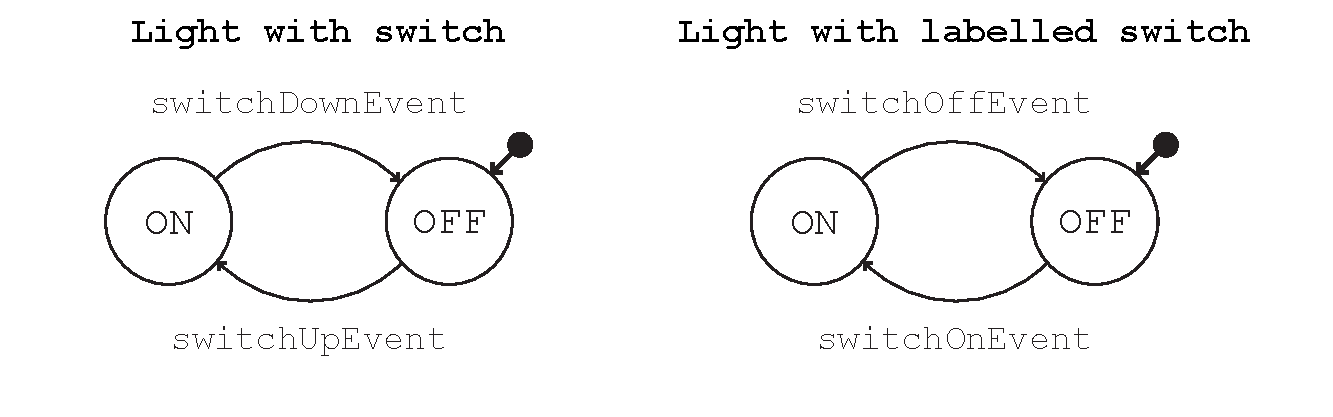
\includegraphics[width=\columnwidth]{FSMsimple}}
\caption{FSMs for a simple light with a switch and a light with a labelled switch}
\label{FSMsimple}
\end{figure}

\begin{figure}
\centerline{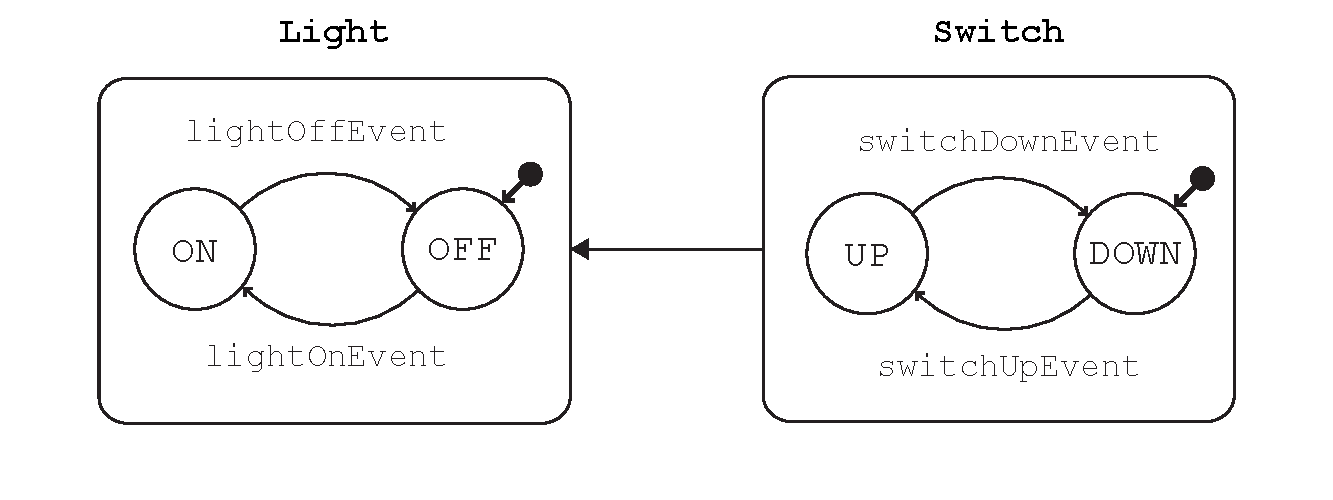
\includegraphics[width=\columnwidth]{FSMsmartObject}}
\caption{Light and light switch as two separate smart objects with a semantic connection}
\label{FSMsmartObject}
\end{figure}

In Figure \ref{FSMsmartObject} one of the simplest examples of a semantic connection is shown - a light (as a smart object) connected to a simple up/down switch (a second smart object). The light consists of two states (\texttt{On/Off}) with an initial (default) state of \texttt{Off}, and two events (\texttt{Light\-On\-Event / Light\-Off\-Event}) indicating the transitions be\-tween these states. Boxes with rounded corners are used to signify smart objects, while the semantic connection is indicated using a solid arrow point. Using arrows to denote semantic connections allows us to specify a direction for the connection. \marginpar{The concept of directionality was described in Section \ref{directionality}.} Note that the light has functional feedback, with perceivable light when it is switched on. The switch on the other hand has inherent feedback, with a perceivable \texttt{Up} or \texttt{Down} state.  

We can create mappings between the events to create an interaction path (see section \ref{interactionPath}), for example we use

\begin{quote}
SwitchUpEvent $\rightarrow$ LightOnEvent %: Default
\end{quote}

to indicate the most meaningful \emph{default} mapping. It should of course be possible to change this mapping, for example by using a semantic transformer that inverts mappings between devices.

\begin{figure}
\centerline{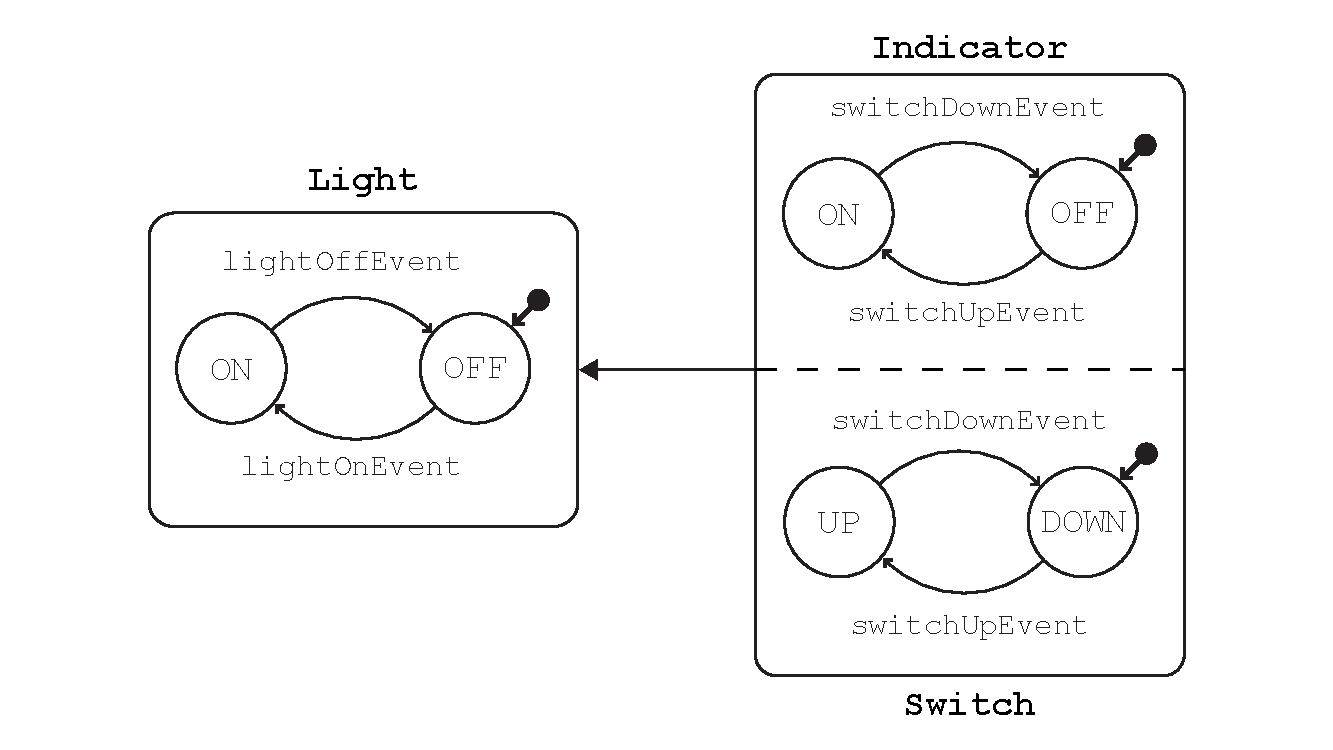
\includegraphics[width=\columnwidth]{FSMaugmentedFeedback}}
\caption{Light connected to light switch with augmented feedback}
\label{FSMaugmentedFeedback}
\end{figure}

In the case where a smart object is not in the same physical location as the smart object it is connected to, additional augmented feedback may be required. Consider the case where the light switch may be in a different room than the light - we could use an indicator on the switch to give augmented feedback to show whether the light actually switched on. This is shown in Figure \ref{FSMaugmentedFeedback}.

\begin{figure}
\centerline{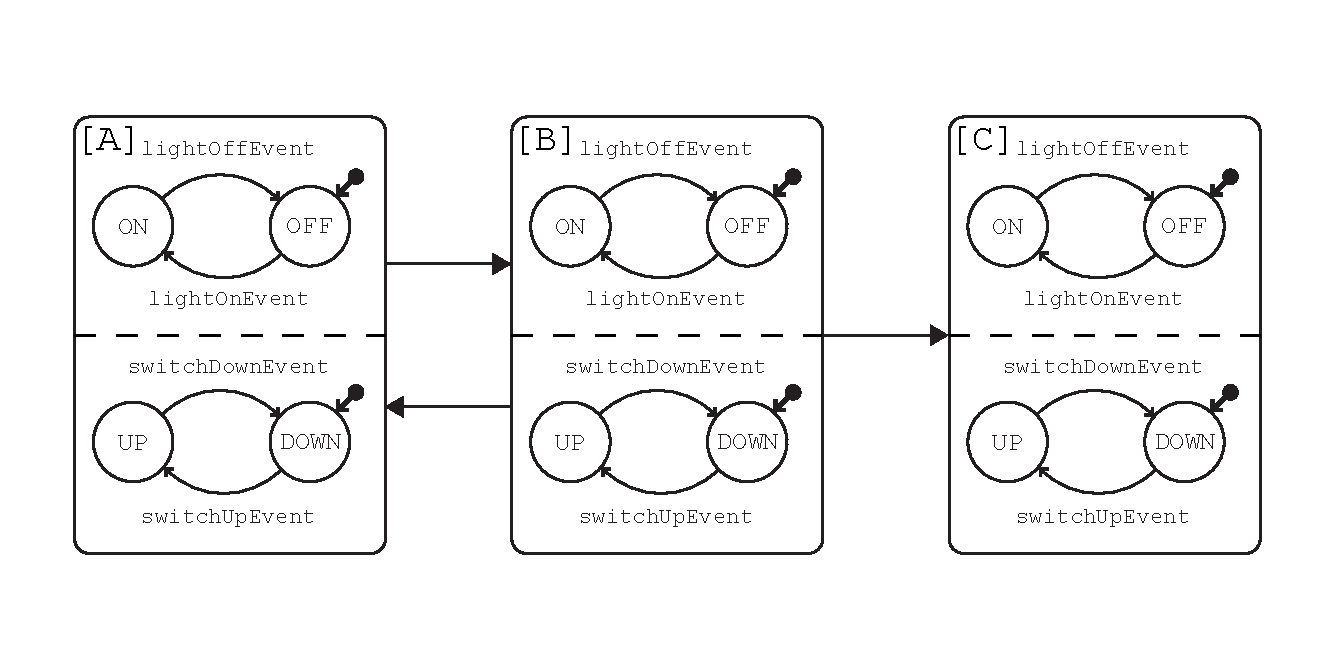
\includegraphics[width=\columnwidth]{FSMsymmetry}}
\caption{FSM showing semantic connection with symmetry}
\label{FSMsymmetry}
\end{figure}

%what about the concept of directionality itself?
A more complex example is shown in Figure \ref{FSMsymmetry}. In this example there is a symmetric (bidirectional) connection between smart object A and B, with the result that pressing the switch on smart object A will turn the light in smart object B either on or off, and vice versa, B will control A. Since B is connected to C, actions on A and B, will also be reflected on C. On the other hand, pressing the switch of C will have no effect on either A or B. Due to the symmetric connection, we expect A and B to be in an identical state. How exactly this is implemented is up to the designer. \marginpar{One possible solution for such a light switch is a push button with an indicator light, such that the switch able to change its state by itself.}
%how does this exactly work with tactile switches with an up/down position, does the switch always change the current state of the connected lights? What about a situation where a physical switch is in an "open" position, and the light is off? does it change the position of the switch? G: I think we consider a smart light switch to not have a permanent "open" position, where the indicator will turn off if the light is off (the position doesn't indicate the state), and the switch will always change the state when pressed.

\begin{figure}
\centerline{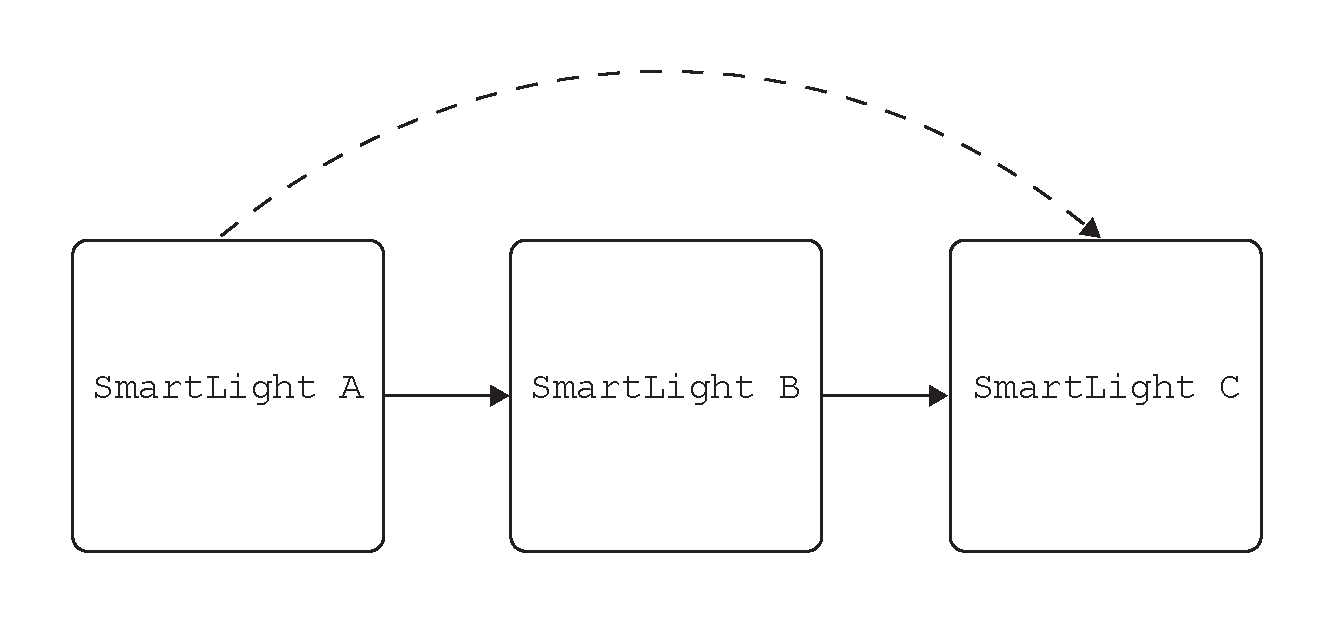
\includegraphics[width=300px]{FSMtransitivity1}}
\caption{FSM showing a semantic connection with transitivity}
\label{FSMtransitivity}
\end{figure}

In Figure \ref{FSMtransitivity} we use the SmartLight abstraction to denote the FSM of a smart light as shown in previous figures. When SmartLight A is connected to SmartLight B, and in turn is connected to C, transitivity allows us to infer a direct connection (indicated by a dashed arrow) between A and C. Pressing the light switch on A will in this case affect both B and C.

\begin{figure}
\centerline{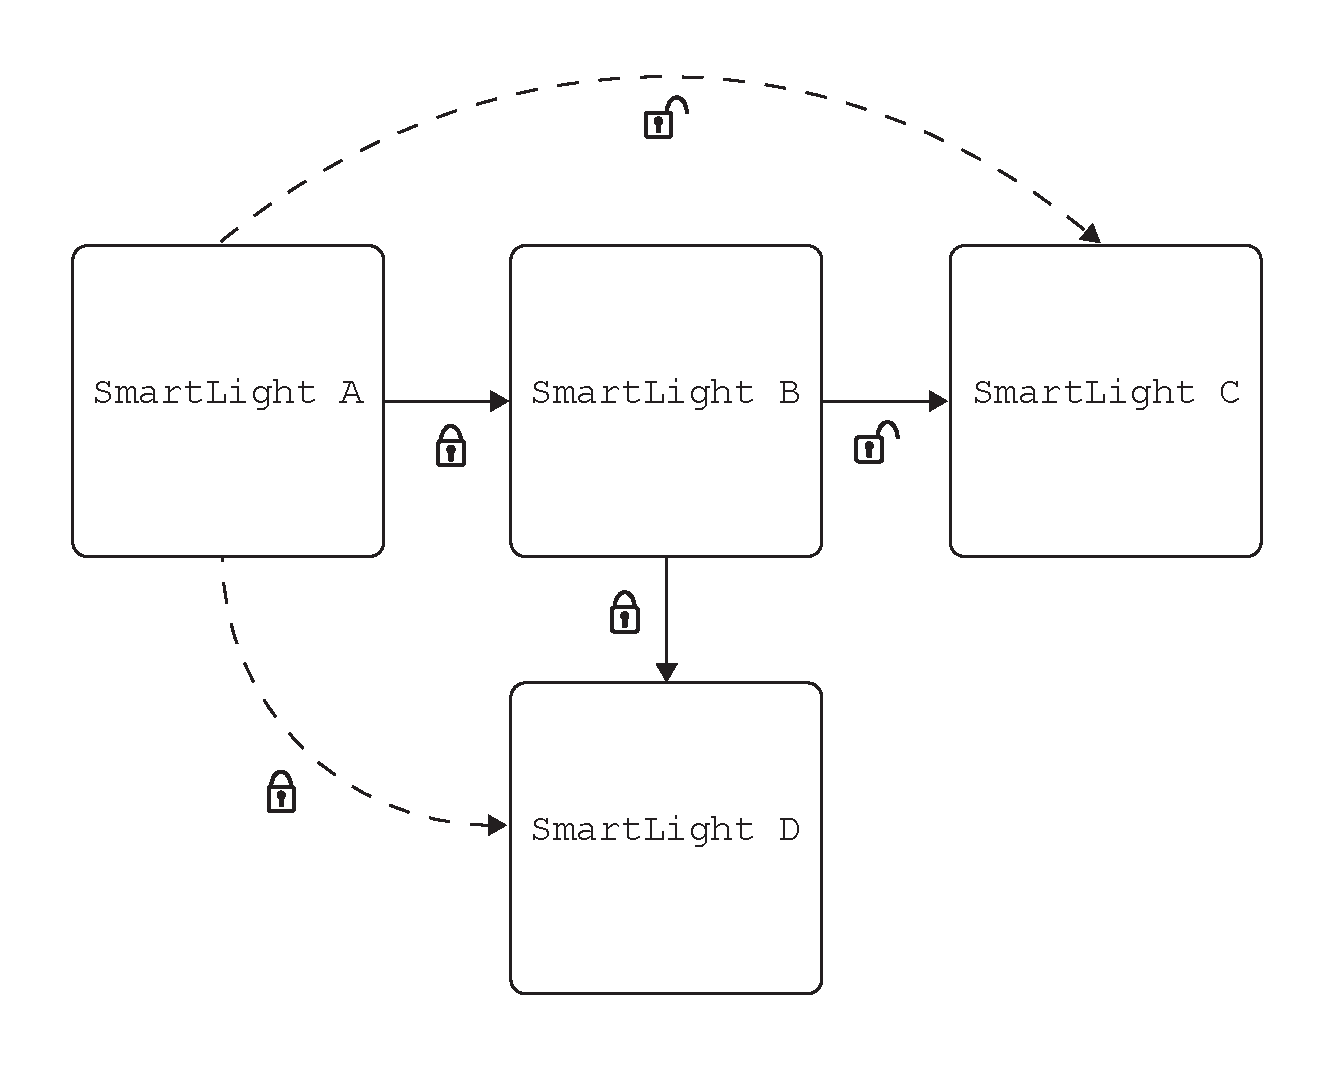
\includegraphics[width=300px]{FSMpersistence}}
\caption{FSM showing a semantic connection with transitivity and persistence}
\label{FSMpersistence}
\end{figure}

We use locked/unlocked icons next to semantic connections to indicate persistence (see Figure \ref{FSMpersistence}). The locked icons between A, B and D indicate persistent connections between those objects, and a persistent transitive connection is then inferred between A and D. This means that if smart object D moves to another location, all three connections (including the A$\rightarrow$D connection) continue to exist. The connection between B and C is temporary, which means that the inferred transitive connection between A and C is also temporary. If smart object C moves to another location, both the B$\rightarrow$C and A$\rightarrow$C connections will be removed.

\begin{figure}
\centerline{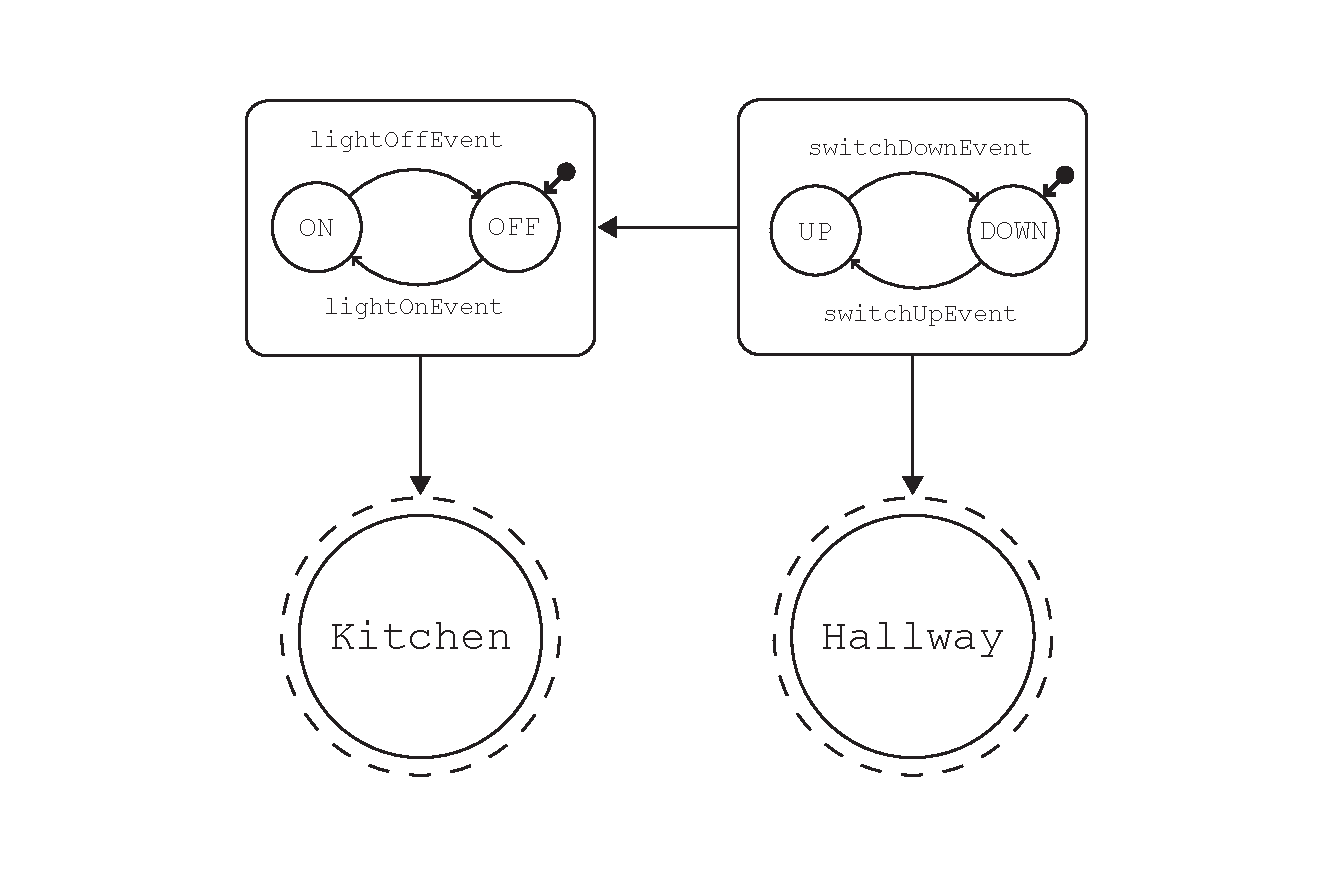
\includegraphics[width=\columnwidth]{FSMplaces}}
\caption{FSM showing semantic connections between smart objects and places}
\label{FSMplaces}
\end{figure}

In Figure \ref{FSMplaces} we show semantic connections between smart objects and specific locations, where the dashed-double circle denotes a location. This places semantic connections between places and objects on the same abstraction level. We use semantic connections between smart objects and places as a way to structure relevant contextual information. In our example in Figure \ref{FSMplaces} we cannot infer that a user actually is able to observe the functional feedback of switching the light on and off, as they are not located in the same space, and might not be able to see the light. The importance of feedback and feedforward and how they should be handled between different locations is described in more detail in section \ref{section:feedbackAndFeedforward}.

\begin{figure}
\centerline{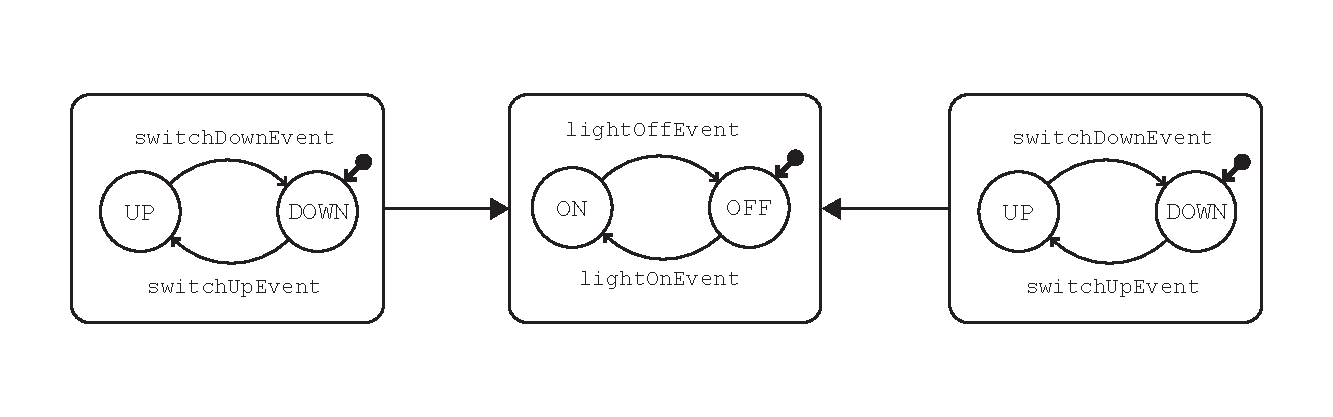
\includegraphics[width=\columnwidth]{FSMpriority}}
\caption{FSM showing a situation where priority is an issue}
\label{FSMpriority}
\end{figure}

When two switches are connected to the same light as is shown in Figure \ref{FSMpriority}, the issue of priority arises. We define the most meaningful default to be that the last event that occurred has priority. In Figure \ref{FSMpresence} where the one interaction is incidental, generated by a presence sensor, and the other is intentional (as described in Section \ref{intentionalSpectrum}), the intentional interaction takes priority.

\begin{figure}
\centerline{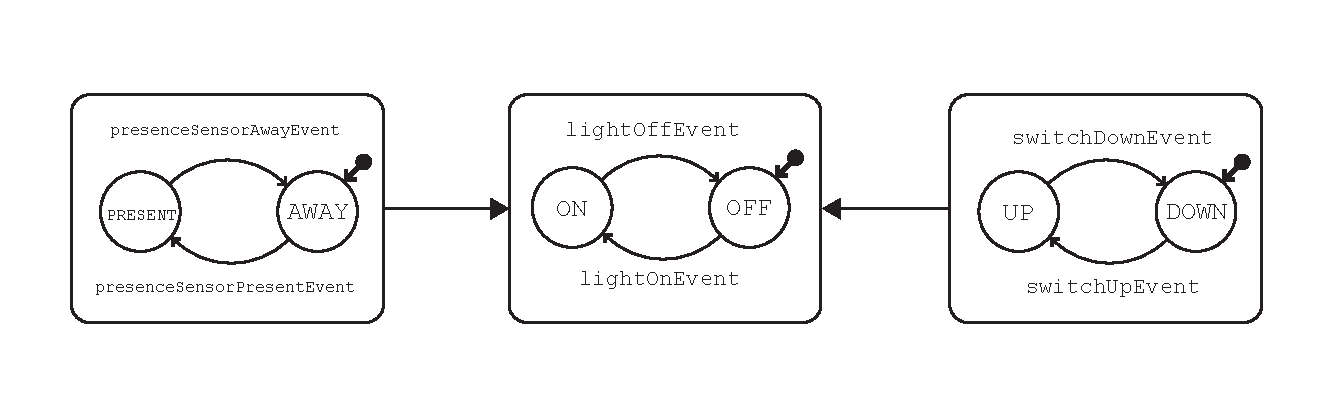
\includegraphics[width=\columnwidth]{FSMpresence}}
\caption{FSM showing incidental (presence sensor) and intentional (light switch) interactions}
\label{FSMpresence}
\end{figure}


\section{Feedback and feedforward}
\label{feedbackforward}
If we view our concept of semantic connections in terms of the Interaction Frogger framework (as discussed in Section \ref{interactionFrogger}), the following interesting insights emerge.

\subsection{Feedback of objects}
When we consider multiple interconnected smart objects and the functionalities and services they provide, information like feedback and feedforward gets spatially distributed. A user may operate a device, receiving inherent feedback locally, but receiving augmented and/or functional feedback remotely. 

As inherent feedback is inherent to the operational controls of the device, these reside only in the physical world and are local to the device. We thus do not model this feedback in the digital domain. Augmented feedback is feedback that is augmented from the digital domain onto the physical world. This type of feedback is subject to change when devices are connected to other devices. In the domain of networked digital artefacts, functional feedback is of a digital nature. Data, media and services that exist in the digital domain become available in the physical world, through the various devices and their connections. In Figure \ref{model}, the several types of feedback are indicated. 

Although many functionalities of digital devices can be regarded as displaying media, data or services, for some simple functionalities this seems problematic. If we, for example, look at functional lighting, it seems that the presence of light as the functionality of a lighting device is not a concept that is part of the digital domain. However, if we view a lighting device as a networked smart object, the presence of lighting, based on some sensor data, can be regarded as the functionality of a digital service.\marginpar{Refer to Van der Vlist's thesis \cite{Bram} for more detail on how the theory of product semantics can be applied to feedback and feedforward.}

% As mentioned before, semantic connections (potentially) \emph{change} functional and augmented feedback and its location. Additionally, semantic connections themselves show feedback as well, when users interact with them through an interaction device. 

\subsection{Feedback of connections}

Inherent feedback becomes feedback that is mediated through an interaction device used to make or break the connection, as one can not manipulate a wireless connection directly. This inherent feedback may however be closely related to the action of making or breaking a physical connection, like a snap or click when the connection is made or broken. Augmented feedback to indicate a connection possibility or an existing connection may be in the form of lights, or in the form of projected or displayed lines. Functional feedback is information about the actual function of the connection, like music playback from a speaker that was just connected to a media player. This type of feedback always reaches the user through the devices being connected. 

\subsection{Feedforward}
Inherent feedforward, conceptually similar to the notion of affordances  \cite{Norman1998}, provides information about the action possibilities with the devices or the individual controls of an interface. Inherent feedforward is always physical and local on the device. However, when devices or objects are part of a larger system, feedforward also emerges where interaction possibilities between objects exist (e.g. a key that fits a lock, a connector of one device or cable that fits another). The same holds for augmented feedforward, where lights, icons, symbols and labels provide additional information about the action possibilities. These may concern the action possibilities locally at the device, as well as action possibilities that concern the interaction with other devices in the environment. 

While inherent and augmented information are primarily concerned with ``the how'', functional feedforward communicates ``the what'', the general function of the device or the function of a control. This type of information often relies on association, metaphors and the sign function of products, and are described in theories such as product semantics and product language. With multifunctional devices, and even more with smart objects, this becomes increasingly difficult. Introducing the concept of semantic connections tries to address these problems, therefore the functional feedforward is the main challenge when designing semantic connections. Functional feedforward gives information about the function of the semantic connection before the interaction takes place. Properly designing functional feedforward is therefore the crucial part of understanding semantic connections, smart services and smart environments.\marginpar{An example of where functional feedforward was used in the third design iteration is described in Section \ref{section:feedbackAndFeedforward}.}

Wensveen \cite{Wensveen2004} further proposes that in interaction, these types of information can link action and function together in time, location, direction, modality, dynamics and expression. Strengthening these couplings between action and function will lead to richer and more intuitive interactions \cite{Wensveen2005}.
 
We can also view semantic connections in the Frogger framework in more general terms. Although semantic connections are not a physical device or product, but rather describe the structure or configuration of a system of devices, the Frogger framework can teach us important lessons. When we look at the link between action and functional information in time or location, a strong link would mean they coincide in time and location. For location this would mean that the connection that is made between devices corresponds to the location of the actual devices in physical space. But also that the feedback that is provided is coupled to the action in time an location. Additionally, the direction of the action of connecting/disconnecting devices, being moving devices towards or away from each other, strengthens the coupling in terms of direction. Also, the direction of the action could have a link to the directionality of the semantic connection that is made (e.g. the order in which endpoints of a connections are defined). Couplings in dynamics (of the action) can be used in similar ways and may express the persistence of the connection that is made. 



\section{Discussion \& Conclusion}

In this chapter we introduced our Semantic Connections theory and used finite state machines to model and explain the different concepts. We defined the following main concepts: 

\begin{itemize}
	\item Smart objects, and the means to describe them in terms of a unique physical and digital identity
	\item Interaction primitives, and how they can be used to describe the user interaction capabilities of smart objects
	\item Semantic connections, and how they can be used to model meaningful connections between smart objects
	\item Semantic transformers, and how they transform information from one type into another
\end{itemize}   %We showed that, even when important interaction events are shared between smart objects, state misalignments will occur. Good practice is to share all important user interaction events and events that cause state changes that are prominently perceivable by users. Using finite state machines to understand such behaviour helps to achieve this.

We identified some of the principles of semantic connections, including directionality and transitivity, as well as permanent and temporary connections. We also identified principles of the various types of feedback and feedforward that are required, not only for connections but also for smart objects.

The importance of being able to uniquely identify smart objects in both the physical and digital space, as well as sharing their interaction capabilities and states, was shown, including how it was grounded in the theory of interaction models by Nielsen, Card and others.

% In our theory we describe semantic connections as meaningful relations that can exist, not only in between smart objects, but also between smart objects, people and places. Although we still believe this is interesting to consider, this did not form part of the actual implementation. It may be interesting for future work, including e.g. relationships between persons (digitally described in social networks) and investigate whether these different types of relationships should be transitive as well (e.g. person A is friends with person B, person A owns device \texttt{a}, and B owns device \texttt{b}, should we infer friendship between \texttt{a} and \texttt{b}? Or, when device \texttt{a} is in the same room as device \texttt{b} and they are touched together, is it safe to infer data can be exchanged over a connection established without passwords? 

We showed how augmented and functional feedback and feedforward can help users to better predict the functional result of the connections they create. Functional and augmented feedback also showed to be key in maintaining the causal links between user action and function, distributed over interconnected smart objects.

A fundamental difficulty encountered during the implementation of the feedback and feedforward (and which is also a big challenge in interoperability in general), is what we call the \emph{awareness paradox}. To foster emergent functionality, efforts are aimed at enabling smart objects to interoperate without their combined functionality being specifically designed. This means that the smart objects are unaware of each other, exchanging information though an information broker. For the users however, it is imperative that smart objects show behaviour as to appear to be aware of each another. 

The way out of the paradox is to make use of proper use of feedback and feedforward that can be generated  at runtime. Since the connections that may be created during use are not known at design time, smart decisions have to be made on how to describe the interaction events and functionalities that are shared. 

By describing feedback and feedforward of the semantic connections as a result of the match in capabilities and functionalities, and having the semantic transformers and sink objects (instead of the source) produce the preview and indicator feedback, we make sure that they are capable of displaying (i.e. in the widest sense of the word, not limited to the visual modality) this feedback. Our reasoning is that, if a sink can be the sink of a functionality, it should also be capable of giving feedforward and feedback for this functionality.\marginpar{Examples of preview events were shown in Chapter \ref{DesignIteration3}.}

%perhaps the simple examples of the awareness of a presence sensor connected to a light. and/or a more complex example with feedback/feedforward.

Moreover we showed that semantic connections and using semantic transformers to create services is an appealing idea, leading to additional and, more importantly, more meaningful functionalities of ensembles of existing devices. This may reduce the number of devices needed in our daily lives by reducing redundant devices.

%After we implemented our theory we feel more confident that we defined a complete set of entities and properties to achieve our goal of creating interoperability between smart objects and to enable users to interact with the objects and the relationships between them at a semantic level. Even though our theory describes how to implement smart objects and provides the necessary core ontology, we believe enough freedom remains for designers and developers to create their own unique objects and interactions. %examples

The theory of semantic connections described in this chapter provides a foundation for modelling user interactions with interoperating smart objects in smart environments, and therewith the possibility to improve the interoperability among them. We considered the notions of feedback and feedforward to enhance perception of connectivity and the perceived causality between user action and feedback.   

In the next part of the thesis, we will look at other concepts and techniques that can be used in smart environments, like device capability modelling and event modelling. Similarly to how we extracted the theory of semantic connections from the work completed in the design iterations, these more general concept and techniques are also based on the work done during the three design iterations.

% Summarising, we made the following observations and changed and/or added to the theory accordingly:
% 
% \begin{itemize}
% \item 	we refined the definition of smart objects; 
% \item 	we refined the definition of semantic transformers and the connections between smart objects and semantic transformers;
% \item 	we implemented direction in the semantic connections and observed its implications on information flow and user interaction;
% \item 	with the directionality and transitivity, smart objects are defined as sources, sinks and bridges, semantic transformers can also be bridges;
% \item 	we implemented augmented and functional feedback and feedforward, introducing \texttt{PreviewEvents} and \texttt{IndicatorEvents}; and
% \item 	we implemented  temporary connections between the connector and smart objects (defining a Connector object as a smart object itself).
% \end{itemize}

% With regards to feedback and feedforward, we made important steps towards defining how this important information is changed when devices are considered in a system of networked objects as opposed to the devices in isolation. We believe that our theory may help other interaction designers and developers to deal with design opportunities and challenges that emerge when designing for interoperability.

%end TiiS


% Possible TODO \section{Interaction primitives}
% 24/08/10, 26/08/10, 27/08/10
% InputToAction: 06/10

